\documentclass{beamer}


\usepackage{amsmath}
\usepackage[style=alphabetic,url=true]{biblatex}
\usepackage{environ}
\usepackage{geometry}
\usepackage{graphicx}
\usepackage{tikz}
\usepackage[T2A]{fontenc}
\usepackage[utf8]{inputenc}
\usepackage[cache=false]{minted}
\usepackage{amsmath}
\usepackage{amsfonts}
\usepackage{amssymb}
\usepackage{calrsfs}
\usepackage{animate}
\usepackage{xmpmulti}


% \usetheme{Bergen}

\usecolortheme{beaver}

\setbeamertemplate{itemize item}[circle]
\setbeamertemplate{itemize subitem}{--}
\addtobeamertemplate{navigation symbols}{}{
  \usebeamerfont{footline}%
  \usebeamercolor[fg]{footline}%
  \hspace{1em}%
  \insertframenumber/\inserttotalframenumber
}
\graphicspath{ {./graphics/} }
\setminted[Python]{
  fontsize=\tiny
}
\BeforeBeginEnvironment{minted}{\medskip}
\AfterEndEnvironment{minted}{\medskip}
\usetikzlibrary{matrix}
\tikzset{
  stack/.style={
    matrix of nodes,
    nodes={
      fill=lightgray,draw,text=black,font=\sffamily\bfseries,
      text height=11pt,text depth=3pt,baseline=center, minimum width=1cm
    },
    column sep=-\pgflinewidth/2
  }
}

\title{
  Біткоїн та криптовалютні технології \\
  Лекція 7: Біткоїн-протокол
}

\author{Юрій Жикін}
\date{20 березня, 2025}

\begin{document}

\frame{\titlepage}

\begin{frame}
  \frametitle{Протокол Bitcoin}
  \begin{itemize}
  \item \textbf{Протокол Bitcoin} - це розподілений протокол, що створює
    \textbf{обмежену кількість} \textbf{цифрових токенів (валюти)}, дозволяє
    \textbf{доведено призначати власність} над цими токенами учасникам
    протоколу, і надає їм можливість \textbf{безповоротно передавати} власність
    над токенами іншим учасникам, запобігаючи при цьому \textbf{подвійному
      витрачанню}.
  \item Попередні спроби створення цифрових валют не могли вирішити проблему
    \textbf{подвійного витрачання} без центрального органу контролю.
  \end{itemize}
\end{frame}

\begin{frame}
  \frametitle{Учасники Біткоїн-протоколу 1/2}
  \begin{itemize}
  \item Учасники Біткоїн-протоколу поділяються на наступні класи:
    \begin{itemize}
    \item \textbf{повноцінні вузли} (вузли перевірки) - учасники, які
      підтримують програмне забезпечення Біткоїн-вузла, яке поширює і перевіряє
      блоки та транзакції; повноцінні вузли забезпечують \textit{``силу в
        кількості''} Біткоїн-мережі;
    \item \textbf{майнери} (повноцінні вузли з обладнанням для майнінгу) -
      учасники, які обчислюють блоки та забезпечують \textit{обчислювальну
        безпеку} мережі;
    \item \textbf{легкі вузли} - вузли, які зацікавлені лише у певними
      компонентах Біткоїн-протоколу, наприклад, у певних транзакціях та блоках,
      в яких вони знаходяться (вузли спрощеної перевірки платежів, програмне
      забезпечення мобільних гаманців).
    \end{itemize}
  \end{itemize}
\end{frame}

\begin{frame}
  \frametitle{Учасники Біткоїн-протоколу 2/2}
  \begin{itemize}
  \item \textbf{Повні вузли} перевіряють, що майнери не генерують недійсних
    блоків (тобто блоків з низькою складністю або блоків з недійсними
    транзакціями);
  \item \textbf{Майнери}
    \begin{itemize}
    \item не можуть генерувати недійсні блоки, оскільки вони будуть негайно
      відхилені повноцінними вузлами, що призведе до повної втрати всіх
      ресурсів, витрачених на обчислення доказу виконаної роботи,
    \item інвестують у обладнання для майнінгу, при цьому їх єдиний дохід - це
      винагорода за нові блоки, тому, якщо безпека мережі буде порушена, їхні
      інвестиції будуть втрачені;
    \end{itemize}
  \item \textbf{Легкі вузли} зберігають лише ланцюг заголовків блоків (68 МіБ
    даних станом на березень 2025 року) і перевіряють лише певні транзакції.
  \end{itemize}
\end{frame}

\begin{frame}
  \frametitle{Обмежена пропозиція 1/4}
  \begin{itemize}
  \item Біткоїн-протокол заохочує майнерів витрачати ресурси на обчислення нових
    блоків, дозволяючи їм присвоювати собі чітко визначену винагороду у так
    званих \textbf{породжуючих транзакціях} (coinbase-транзакціях).
  \item Крім того, майнер отримує комісію з усіх транзакцій, які були включені в
    блок.
  \item Однією з фундаментальних властивостей Біткоїн-системи є \textbf{строго
      обмежена пропозиція} валюти, тому кількість біткоїнів, що генеруються в
    кожному новому блоці, зменшується з часом.
  \item Зі зменшенням винагороди за блоки майнери все більше залежать від
    комісій за транзакції.
  \end{itemize}
\end{frame}

\begin{frame}
  \frametitle{Обмежена пропозиція 2/4}
  \begin{itemize}
  \item Кожні 210 000 блоків винагорода зменшується вдвічі:
    \begin{itemize}
    \item 50 BTC (5 000 000 000 сатоші) у 2009-2012 роках,
    \item 25 BTC (2 500 000 000 сатоші) у 2012-2016 роках,
    \item 12.5 BTC (1 250 000 000 сатоші) у 2016-2020 роках,
    \item 6.25 BTC (625 000 000 сатоші) у 2020-2024 роках,
    \item 3.125 BTC (312 500 000 сатоші) з 2024 року.
    \end{itemize}
  \item Винагорода за блок слідує геометричній прогресії:
    $$a_n = ar^n \text{, } a = 50 \text{, } r = \frac{1}{2}$$
    сума якої визначає загальну кількість біткоїнів, які коли-небудь
    існуватимуть:
    $$210000 \times \sum_{n = 1}^{n: a_n \geq 1} a_n = 210000 \times \frac{a(1 -
      r^n)}{1 - r} = 21000000$$
  \end{itemize}
\end{frame}

\begin{frame}
  \frametitle{Обмежена пропозиція 3/4}
  \begin{itemize}
  \item Біткоїни можуть бути випадково ``втрачені'' (якщо власник втрачає доступ
    до ключа, необхідного для розблокування скрипта блокування).
  \item Біткоїни також можуть бути навмисно ``знищені'' шляхом надсилання монет
    на адресу з невідомим ключем, наприклад:
    \begin{small}
      $$1BitcoinEaterAddressDontSendf59kuE$$
    \end{small}
  \item За деякими дослідженнями, приблизно 600000-1100000 біткоїнів можуть
    належати Сатоші Накамото ще з раннього періоду існування мережі.
  \end{itemize}
\end{frame}

\begin{frame}
  \frametitle{Обмежена пропозиція 4/4}
  \begin{itemize}
  \item \href{https://bitcoinisdata.com}{bitcoinisdata.com}: 4-6 мільйонів
    біткоїнів, ймовірно, втрачено назавжди.
  \end{itemize}
  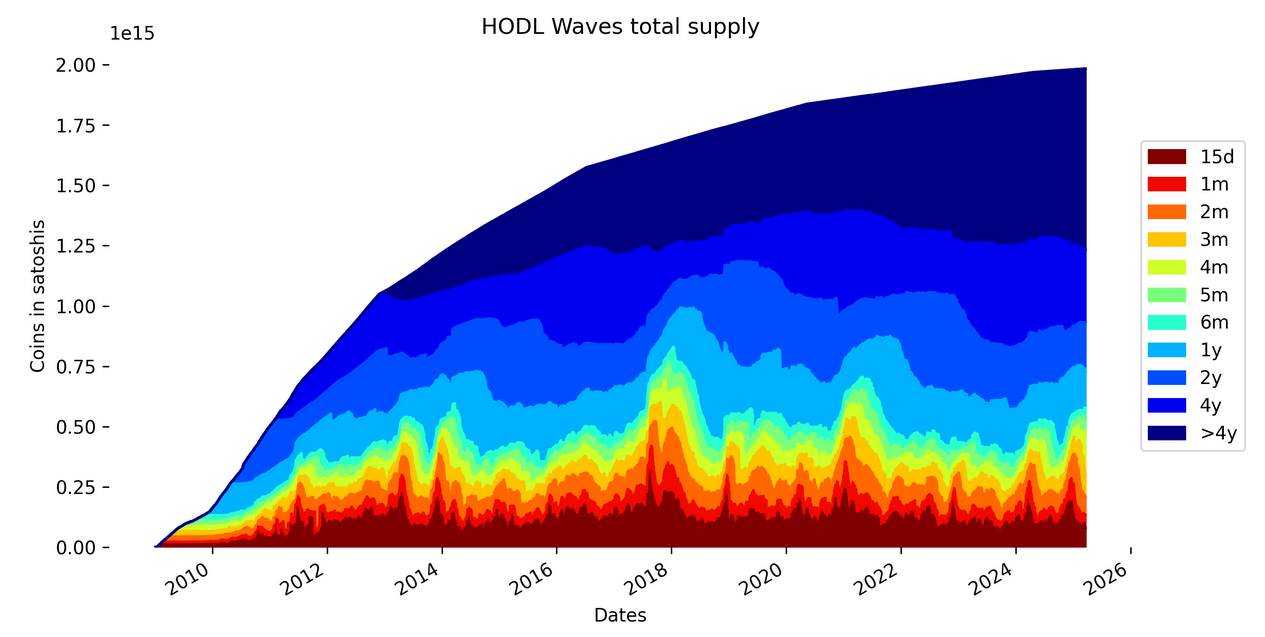
\includegraphics[width=\textwidth]{utxo-age}
\end{frame}

\begin{frame}
  \frametitle{Розгалуження 1/2}
  \begin{itemize}
  \item \textbf{М'яке розгалуження (софтфорк)} - це зміна Біткоїн-протоколу, яка
    \textbf{обмежує} набір правил консенсусу, що застосовуються при валідації
    блоків і транзакцій.
  \item \textbf{Деякі} блоки або транзакції, які вважалися \textbf{дійсними}
    \textbf{старими (неоновленими) вузлами}, вважаються \textbf{недійсними}
    \textbf{новими (оновленими) вузлами}.
  \item М'яке розгалуження не виключає вузли з консенсусу і не розколює мережу,
    але для забезпечення дії нового правила потребує, щоб більшість вузлів
    оновилися.
  \item Старі вузли можуть продовжувати ``грати за старими правилами''.
  \end{itemize}
\end{frame}

\begin{frame}
  \frametitle{Форки 2/2}
  \begin{itemize}
  \item \textbf{Жорстке розгалуження (хардфорк)} - це зміна Біткоїн-протоколу,
    яка \textbf{послаблює} набір правил консенсусу, що застосовуються при
    валідації блоків і транзакцій.
  \item \textbf{Деякі} блоки або транзакції, які вважаються \textbf{дійсними}
    \textbf{новими (оновленими) вузлами}, вважаються \textbf{недійсними}
    \textbf{старими (неоновленими) вузлами}.
  \item Жорстке розгалуження фактично виключає старі вузли з консенсусу, тому
    воно вимагає, щоб усі вузли оновилися, щоб уникнути розколу мережі.
  \item Вузли, які ``грають за старими правилами'', відокремлюються від основної
    мережі у окрему мережу.
  \end{itemize}
\end{frame}

\begin{frame}
  \frametitle{Обчислювальна потужність мережі 1/2}
  \begin{itemize}
  \item Для \textbf{систем на основі доказу роботи (Proof-of-Work)},
    обчислювальну потужність зручно вимірювати \textbf{хешрейтом} -
    \textbf{кількістю операцій хешування, які мережа здійснює за секунду} (х/с).
  \item Оскільки зростання винагороди за блоки зі зростанням вартості біткоїна
    приваблює все більше майнерів, зростає і загальна обчислювальна потужність
    Біткоїн-мережі.
  \item Поточний загальний \textbf{хешрейт} Біткоїн-мережі становить приблизно
    804 Ех/c ($804 \times 10^{18} = $ 804,000,000,000,000,000 х/с), у порівнянні
    з 375 Ех/с у 2022 році.
  \end{itemize}
\end{frame}

\begin{frame}
  \frametitle{Обчислювальна потужність мережі 2/2}
  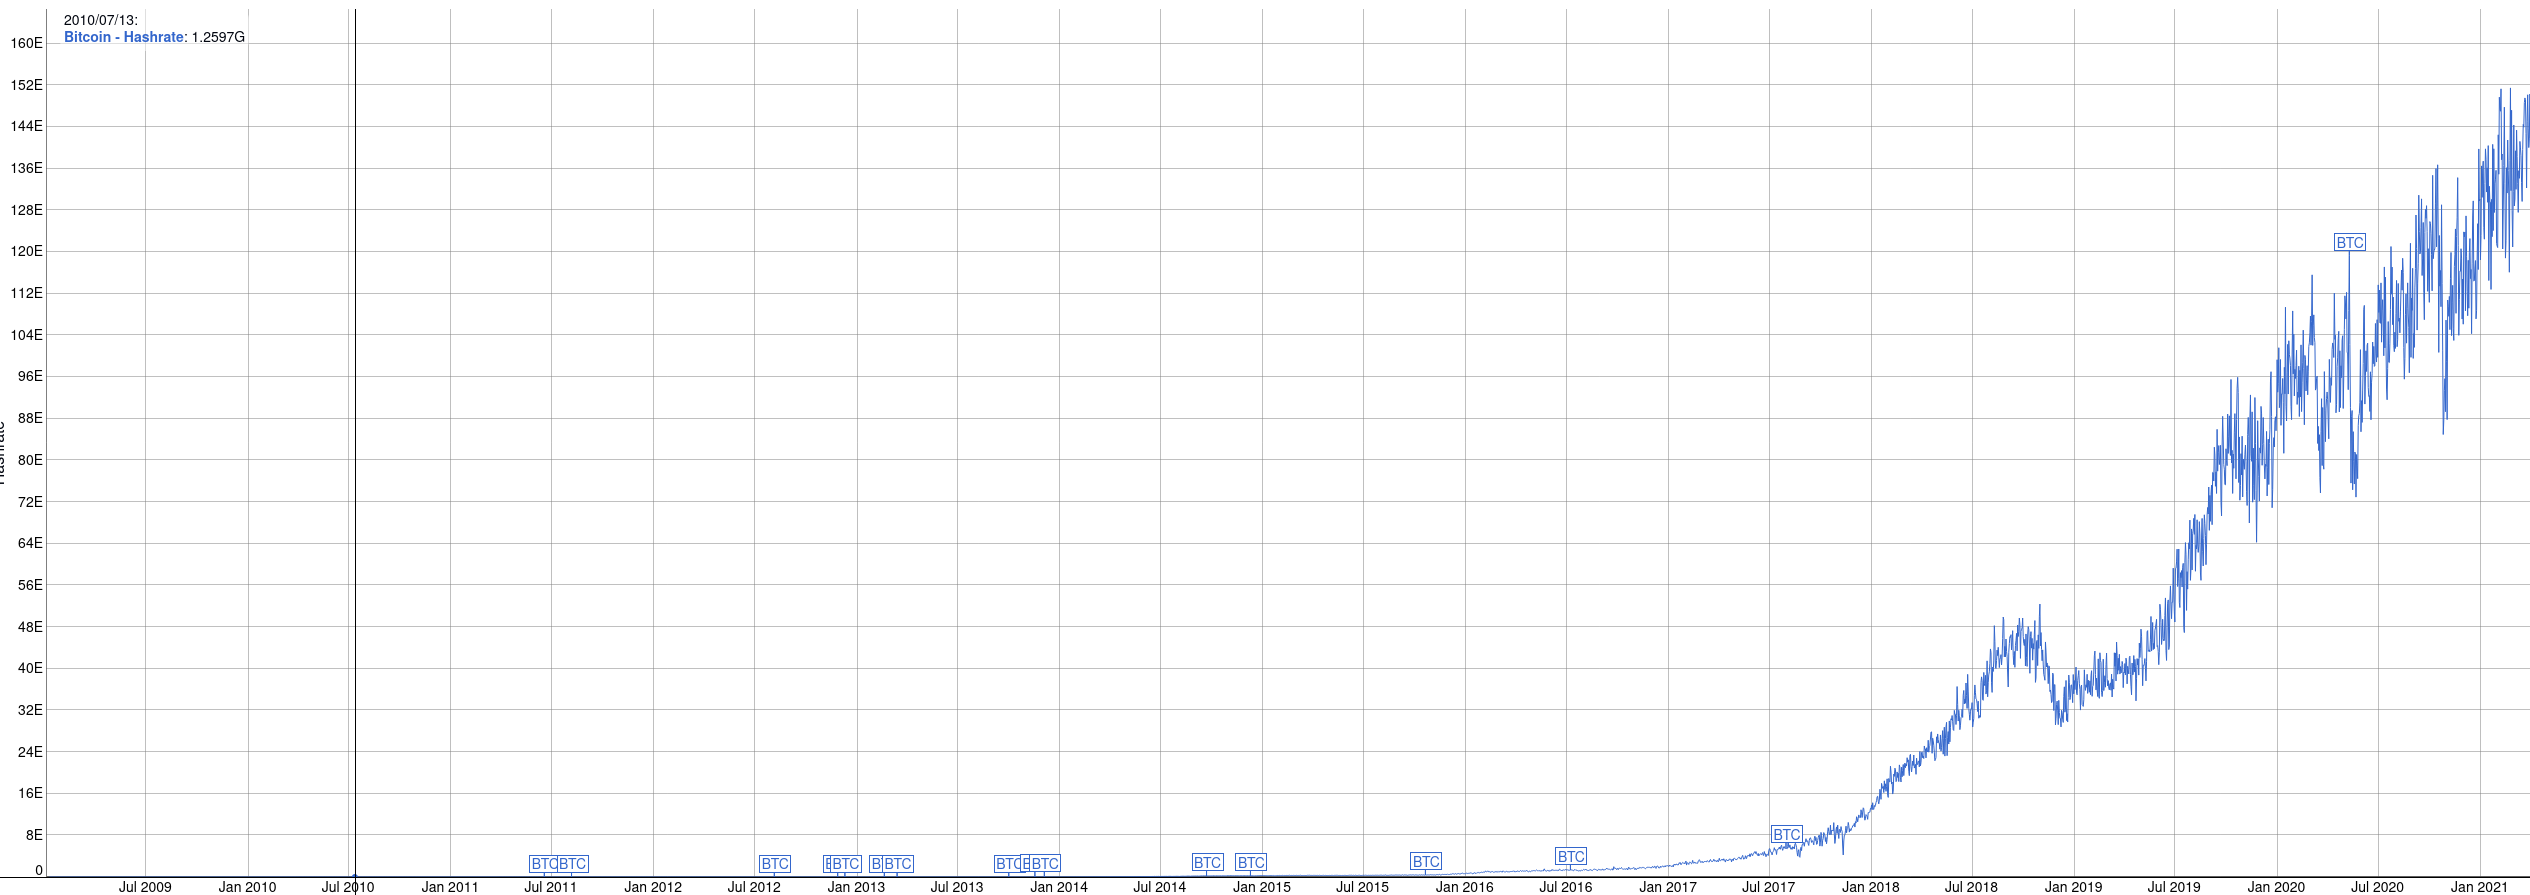
\includegraphics[width=\textwidth]{hashrate}
\end{frame}

\begin{frame}
  \frametitle{Коригування складності}
  \begin{itemize}
  \item Для того, щоб адаптуватись до зростаючої обчислювальної потужності
    мережі, Біткоїн-протоколі існує механізм \textbf{коригування складності}.
  \item Кожні 2016 блоків (приблизно кожні 2 тижні) складність задачі доказу
    виконаної роботи перераховується на основі останніх 2016 блоків:
    \begin{itemize}
    \item якщо середній час між цими 2016 блоками \textit{більший за 600
        секунд}, \textit{складність зменшується} (\textit{цільове число
        збільшується}), інакше \textit{складність збільшується} (\textit{цільове
        число зменшується}).
    \end{itemize}
  \item Складність PoW представляється у вигляді \textbf{цільового числа} -
    256-бітного числа, яке, у свою чергу, перетворюється у значення
    \textbf{bits} і включається у заголовок блоку, щоб доказ виконаної роботи
    міг бути перевірений незалежно для окремого блока.
  \end{itemize}
\end{frame}

\begin{frame}
  \frametitle{Кінець}
  \begin{center}
    Дякую за увагу!
  \end{center}
\end{frame}

\end{document}

%%% Local Variables:
%%% mode: latex
%%% TeX-master: t
%%% End:
